\chapter{Πειράματα - Αποτελέσματα}
\label{chapter:experiments}

Τα πειράματα χωρίζονται σε δύο φάσεις. Η πρώτη αναφέρεται στην εκτέλεση
της διαδικασίας προς-τα-εμπρός περάσματος (forward propagation) στο εκάστοτε
CNN, σε PC με επεξεργαστή \emph{Intel i7 6700}.
Στην δεύτερη φάση οι υλοποιήσεις εκτελέστηκαν χρησιμοποιώντας
ενσωματωμένο σύστημα Jetson TK1.

Κατά την διαδικασία των πειραμάτων μετρήθηκαν τα εξής μεγέθη:
\begin{itemize}
  \item{Απαιτούμενη κατά την εκτέλεση μνήμη RAM}
  \item{Χρόνος εκτέλεσης της διαδικασίας \emph{forward propagation}}
  \item{Κατανάλωση ισχύος (για την πλατφόρμα Jetson TK1)}
\end{itemize}

Η μέτρηση της ισχύος που καταναλώνει η πλακέτα έγινε ακολουθώντας την παρακάτω μεθοδολογία:
\begin{itemize}
  \item{Από το έγγραφο που περιγράφει τα σχηματικά της πλακέτας \footnote{TK1 Compact Development Module,  602-7R375-0000-D10, σελίδα 27}
    βρέθηκε η αντίσταση (R5C11, 5mΩ) από την οποία περνάει το ρεύμα που παρέχεται από το τροφοδοτικό.}
  \item{Βρέθηκε πάνω στην πλακέτα η θέση της αντίστασης και χρησιμοποιήθηκε ένα
    πολύμετρο για λήψη της τιμής της τάσης στα άκρα της.
    Από την τιμή της αντίστασης και της τάσης στα άκρα της υπολογίζεται το ρεύμα που διέρχεται από αυτήν,
    το οποίο ισοδυναμεί με το ρεύμα που λαμβάνει η πλακέτα από το τροφοδοτικό.}
  \item{Γνωρίζοντας την τιμή της τάσης τροφοδοσίας (12.15Volts) και την τιμή
    του ρεύματος που λαμβάνεται από το τροφοδοτικό, υπολογίζεται η παρεχόμενη στην πλακέτα ισχύ.}
\end{itemize}

Προτού γίνουν μετρήσεις ισχύος, χρησιμοποιήθηκε το εργαλείο \emph{powertop}\footnote{PowerTOP: \url{https://github.com/fenrus75/powertop}},
το οποίο δίνει πληροφορίες σχετικά με τις ενεργοποιημένες μονάδες ενός συστήματος
και την σχετική απόδοσή τους σε κατανάλωση ισχύος (όχι σε τιμές Watt).
Οι πιο κάτω προτάσεις του συγκεκριμένου εργαλείου για το
ενσωματωμένο σύστημα Jetson TK1 λήφθηκαν υπόψη:
\begin{itemize}
  \item{Απενεργοποίηση των ελεγκτών USB (EHCI και xHCI).}
  \item{Ενεργοποίηση λειτουργίας διαχείρισης ισχύος για τον ελεγκτή SATA (SATA link power managment)}
  \item{Ενεργοποίηση λειτουργίας διαχείρισης ισχύος της μονάδας Audio Codec (Audio Codec power managment)}
  \item{Ενεργοποίηση λειτουργίας διαχείρισης ισχύος διαύλου PCIe (PCIe bridge runtime power managment)}
\end{itemize}

Στην συνέχεια μετρήθηκε η τιμή της κατανάλωσης ισχύος της πλακέτας σε κατάσταση αεργίας (idle),
στα $3.4$Watts. Σημαντικό επίσης να αναφερθεί ότι ο ανεμιστήρας τον οποίο
διαθέτει το συγκεκριμένο ενσωματωμένο, για την ψύξη του SOC, καταναλώνει $0.85$Watts
\footnote{Κατανάλωσης ισχύος του ανεμιστήρα που διαθέτει το Jetson TK1 \url{http://elinux.org/Jetson/Graphics_Performance\#Test_Methodology}}.

Για λόγους πληρότητας, πιο κάτω παρουσιάζονται τα βασικά χαρακτηριστικά
των δύο συστημάτων που χρησιμοποιήθηκαν στην εκτέλεση των πειραμάτων:
\begin{center}
\small
\begin{tabular}{ | l | l | l | l | l | l | l | }
  \hline
  \rowcolor{Gray}
  Μηχάνημα & \# πυρήνων & \# νημάτων & clock & Κατ. Ισχύος & RAM & Cache \\
  \hline
  Host PC & 4 & 8 & 3.4 Ghz & ~65Watts & 16GB & 8MΒ L3 \\
  \hline
  TK1 & 4 & 4 & 2.32 Ghz & ~12Watts & 2GB (shared) & 2MB L2 \\
  \hline
\end{tabular}
\end{center}

Ο αριθμός νημάτων (8) που υποστηρίζει ο επεξεργαστής i7-6500 οφείλεται στην
τεχνολογία \emph{Hyper-Threading}\footnote{\url{http://www.intel.com/content/www/us/en/architecture-and-technology/hyper-threading/hyper-threading-technology.html}}.
Επίσης, η τιμή της κατανάλωσης ισχύος για την
πλατφόρμα Jetson TK1, αντιστοιχεί στην κατάσταση μέγιστης (ταυτόχρονης) λειτουργίας των μονάδων
CPU και GPU.

\section{Πρώτη Φάση Πειραμάτων}
\label{sec:experiments_phase1}

Οι μετρήσεις κατανάλωσης ισχύος στον επεξεργαστή Intel-i7-6700 έγιναν
χρησιμοποιώντας το εργαλείο \emph{PowerAPI} \cite{grant2016standardizing}.
Το τελευταίο, επιτρέπει την μέτρηση κατανάλωσης ισχύος σε
επίπεδο διεργασίας (process). Για την βέλτιστη λειτουργία του,
απαιτείται η ρύθμιση της παραμέτρου TDP (Thermal Design Power) για τον εκάστοτε
επεξεργαστή στον οποίο λαμβάνονται οι μετρήσεις. Η τιμή αυτής της παραμέτρου για τον επεξεργαστή
Intel-i7-6700, θεωρήθηκε στα 65W σύμφωνα με το αντίστοιχο τεχνικό εγχειρίδιο
\footnote{Intel i7 6700 TDP: \url{http://ark.intel.com/products/88196/Intel-Core-i7-6700-Processor-8M-Cache-up-to-4_00-GHz}}.
Επιπρόσθετα, για τις μετρήσεις που πραγματοποιήθηκαν λήφθηκαν υπόψη οι εξής παράγοντες:
\begin{itemize}
  \item{Δυναμική κατανάλωση ισχύος που οφείλεται στην δραστηριότητα των λογικών πυλών του επεξεργαστή}
  \item{Κατανάλωση ισχύος ανοικτού κυκλώματος (short-circuit)}
  \item{Απώλειες ισχύος λόγω διαρροής ρεύματος στα τρανζίστορ του επεξεργαστή (transistor leakage currents)}
\end{itemize}

Αρχικά μετρήθηκε η τιμή της κατανάλωσης ισχύος (μέγιστη) του επεξεργαστή σε
κατάσταση αεργίας (idle), στα $3.66$Watt.

Οι εκδόσεις των εργαλείων λογισμικού που χρησιμοποιήθηκαν
κατά την διάρκεια των πειραμάτων για τον επεξεργαστή Intel-i7-6700 είναι:
\begin{itemize}
  \item{Keras: v1.1.0}
  \item{Theano: v0.9.0-dev3}
  \item{numpy: v1.12.0}
  \item{scipy: v0.19.0-dev0}
\end{itemize}


% --------------------------------------------------------------------------

\subsection{AlexNet}

Οι παράμετροι των πειραμάτων είναι οι εξής:
\begin{itemize}
  \item{Αριθμός επαναλήψεων: 1000}
  \item{Αριθμός Νημάτων: 1, 2, 4, 8}
\end{itemize}

Στον \autoref{tab:alexnet_i7} παρουσιάζονται τα αποτελέσματα της μέσης τιμής
του χρόνου εκτέλεσης, ενώ στο \autoref{fig:alexnet_results_i7} φαίνεται
το διάγραμμα του χρόνου εκτέλεσης σε κάθε επανάληψη.

\begin{table}[H]
  \begin{center}
    \caption{Μετρήσεις πειραμάτων για το δίκτυο AlexNet σε επεξεργαστή Intel-i7-6700}
    \label{tab:alexnet_i7}
    \begin{tabular}{ | c | c | c | c | }
      \hline
      \rowcolor{Gray}
      \# νημάτων & Χρόνος Εκτέλεσης (sec) & Κατανάλωση Ισχύος (Watts) & Perf / Watt \\
      \hline
      1 & $0.117$ & $8.21$ & $1.04$ \\
      2 & $0.095$ & $16.43$ & $0.64$ \\
      4 & $0.095$ & $32.62$ & $0.32$ \\
      8 & $0.127$ & $58.84$ & $0.13$ \\
      \hline
    \end{tabular}
  \end{center}
\end{table}

Η μέγιστη τιμή μνήμης RAM που δεσμεύει το δίκτυο AlexNet μετρήθηκε στα \emph{692MB}.
\newpage

\begin{figure}[H]
  \centering
  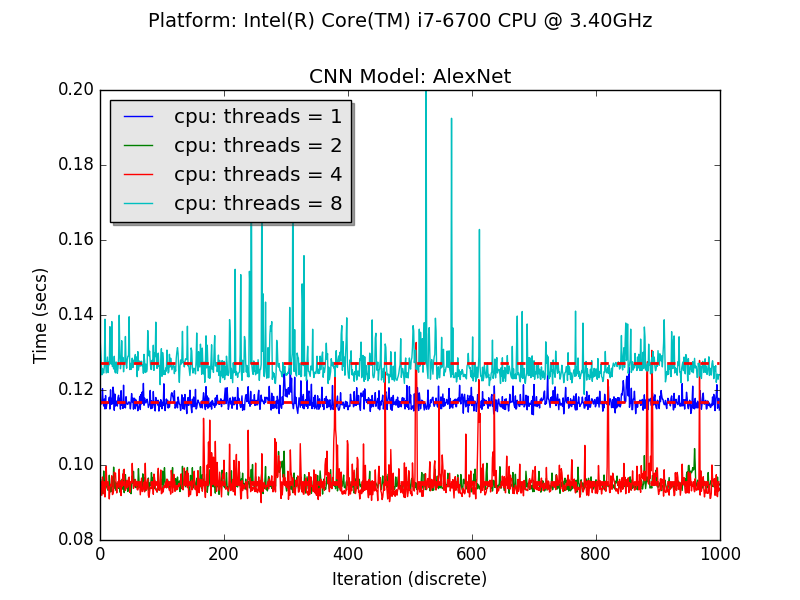
\includegraphics[width=0.8\textwidth]{./images/chapter6/benchmark_alexnet_i7.png}
  \caption[Χρόνoι εκτέλεσης για το δίκτυο AlexNet σε επεξεργαστή i7]{Χρόνοι εκτέλεσης για το δίκτυο AlexNet σε επεξεργαστή i7}
  \label{fig:alexnet_results_i7}
\end{figure}



%%----------------------------------------------------------------------------

\subsection{VGG16}

Οι παράμετροι των πειραμάτων είναι οι εξής:
\begin{itemize}
  \item{Αριθμός επαναλήψεων: 100}
  \item{Αριθμός Νημάτων: 1, 2, 4, 8}
\end{itemize}

Η μέσες τιμές του χρόνου εκτέλεσης των πειραμάτων παρουσιάζονται στον \autoref{tab:vgg16_i7}.
Η απαιτούμενη τιμή μνήμης RAM μετρήθηκε στα \emph{710MB}.

\begin{table}[H]
  \begin{center}
    \caption{Μετρήσεις πειραμάτων για το δίκτυο VGG16 σε επεξεργαστή Intel-i7-6700}
    \label{tab:vgg16_i7}
    \begin{tabular}{ | c | c | c | c | }
      \hline
      \rowcolor{Gray}
      \# νημάτων & Χρόνος Εκτέλεσης (sec) & Κατανάλωση Ισχύος (Watts) & Perf / Watt \\
      \hline
      1 & $0.7709$ & $5.76$ & $0.225$ \\
      2 & $0.5577$ & $11.13$ & $0.161$ \\
      4 & $0.4734$ & $21.05$ & $0.1$ \\
      8 & $0.6555$ & $41.56$ & $0.036$ \\
      \hline
    \end{tabular}
  \end{center}
\end{table}

\begin{figure}[H]
  \centering
  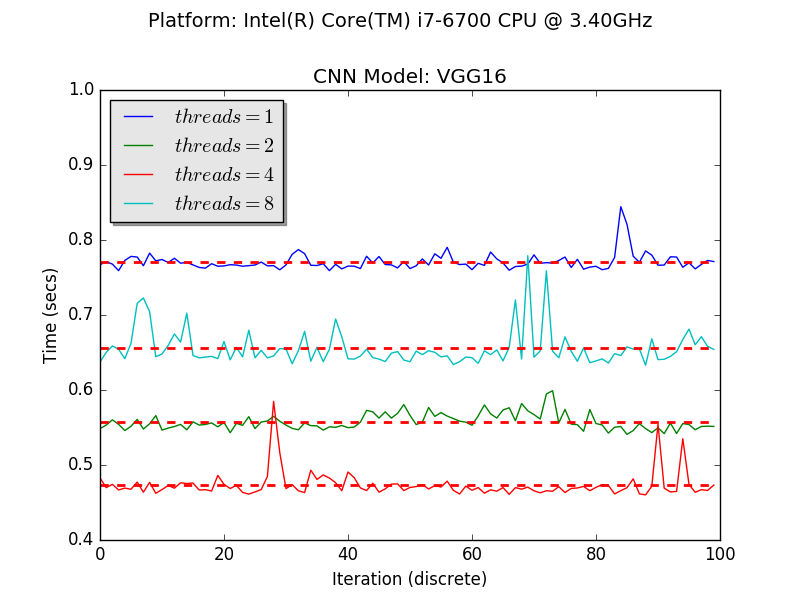
\includegraphics[width=0.8\textwidth]{./images/chapter6/benchmark_vgg16_i7.png}
  \caption[Χρόνoι εκτέλεσης για το δίκτυο VGG16 σε επεξεργαστή i7]{Χρόνοι εκτέλεσης για το δίκτυο VGG16 σε επεξεργαστή i7}
  \label{fig:vgg16_results_i7}
\end{figure}



%%----------------------------------------------------------------------------

\subsection{Tiny-YOLO}

Οι παράμετροι των πειραμάτων είναι οι εξής:
\begin{itemize}
  \item{Αριθμός επαναλήψεων: 1000}
  \item{Αριθμός Νημάτων: 1, 2, 4, 8}
\end{itemize}

Η αντίστοιχη μέση τιμή των χρόνων εκτέλεσης των πειραμάτων παρουσιάζονται στον \autoref{tab:yolo_i7}.
Σημαντικό να αναφερθεί ότι ο χρόνος εκτέλεσης της αντίστοιχης υλοποίησης της ερευνητικής ομάδας
που σχεδίασε το δίκτυο Tiny-YOLO, μετρήθηκε στα \emph{1.096 δευτερόλεπτα} (δεν χρησιμοποιούνται νήματα).

\begin{table}[H]
  \begin{center}
    \caption{Μετρήσεις πειραμάτων για το δίκτυο Tiny-YOLO σε επεξεργαστή Intel-i7-6700}
    \label{tab:yolo_i7}
    \begin{tabular}{ | c | c | c | c | }
      \hline
      \rowcolor{Gray}
      \# νημάτων & Χρόνος Εκτέλεσης (sec) & Κατανάλωση Ισχύος (Watts) & Perf / Watt \\
      \hline
      1 & $0.1871$ & $5.74$ & $0.93$ \\
      2 & $0.1609$ & $11.5$ & $0.54$ \\
      4 & $0.1516$ & $22.86$ & $0.288$ \\
      8 & $0.2309$ & $42.77$ & $0.1$ \\
      \hline
    \end{tabular}
  \end{center}
\end{table}
Η μνήμη (μέγιστη) που απαιτείται κατά την διαδικασία
προς-τα-εμπρός εκτέλεσης μετρήθηκε στα \emph{379MB}.

\begin{figure}[H]
  \centering
  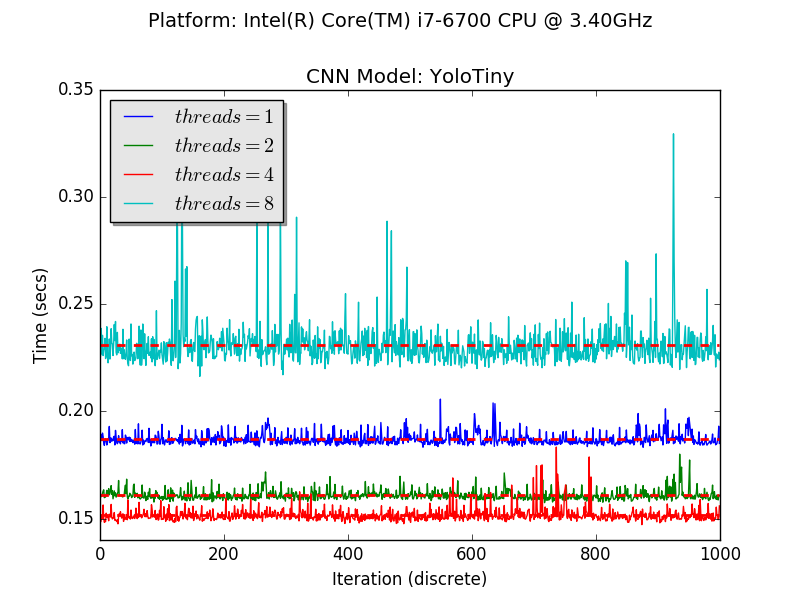
\includegraphics[width=0.8\textwidth]{./images/chapter6/benchmark_yolotiny_i7.png}
  \caption[Χρόνoι εκτέλεσης για το δίκτυο Tiny-YOLO σε επεξεργαστή i7]{Χρόνοι εκτέλεσης για το δίκτυο Tiny-YOLO σε επεξεργαστή i7}
  \label{fig:yolotiny_results_i7}
\end{figure}



\section{Δεύτερη Φάση Πειραμάτων}
\label{sec:experiments_phase2}

Η μεταγλώττιση των δικτύων AlexNet και VGG16 απαιτεί περισσότερη
μνήμη από αυτή που διαθέτει το ενσωματωμένο σύστημα Jetson TK1 (1888MB).
Το πρόβλημα αυτό το αντιμετωπίστηκε προσθέτοντας 1GB μνήμη
\emph{Swap}\footnote{Δημιουργία αρχείου μνήμης swap: \url{http://www.jetsonhacks.com/2014/10/04/creating-swapfile-ubuntu-nvidia-jetson-tk1/}}.

%%----------------------------------------------------------------------------

\subsection{AlexNet}

Οι παράμετροι των πειραμάτων είναι οι εξής:
\begin{itemize}
  \item{Αριθμός επαναλήψεων: 100}
  \item{Υπολογιστική μονάδα:}
    \begin{itemize}
      \item{CPU: Αριθμός Νημάτων (1, 2, 4, 8)}
      \item{GPU: Με και χωρίς εκ των προτέρων δέσμευση μνήμης}
    \end{itemize}
\end{itemize}

\begin{figure}[H]
  \centering
  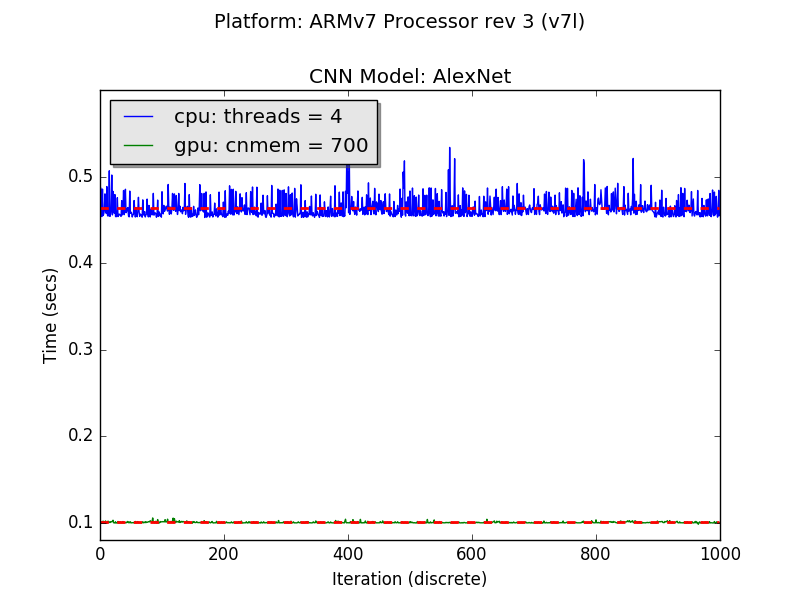
\includegraphics[width=0.8\textwidth]{./images/chapter6/benchmark_alexnet_jetson.png}
  \caption[Χρόνoι εκτέλεσης για το δίκτυο AlexNet στο Jetson TK1]{Χρόνoι εκτέλεσης για το δίκτυο AlexNet στο Jetson TK1}
  \label{fig:alexnet_results_jetson}
\end{figure}

Στον \autoref{tab:alexnet_jetson} παρουσιάζονται τα συγκριτικά αποτελέσματα της
εκτέλεσης τόσο στην μονάδα CPU (με μεταβλητό αριθμό νημάτων), όσο και στην
GPU (με και χωρίς εκ των προτέρων δέσμευση μνήμης).

\begin{table}[H]
  \begin{center}
    \caption{Μετρήσεις πειραμάτων για το δίκτυο AlexNet στο Jetson TK1}
    \label{tab:alexnet_jetson}
    \small
    \begin{tabular}[center]{ | c | c | c | c | c | }
      \hline
      \rowcolor{Gray}
      Υπολ. Μονάδα & \# νημάτων & cnmem & Χρόνος εκτέλεσης (sec) & Κατ. Ισχύος (Watts) \\
      \hline
      CPU & 1 & N/A & 0.62 & 6.318\\
      CPU & 2 & N/A & 0.4845 & 8.019\\
      CPU & 4 & N/A & 0.4634 & 10.692\\
      CPU & 8 & N/A & 0.4646 & 10.692\\
      GPU & N/A & None & 0.1049 & 8.5\\
      GPU & N/A & 700MB & 0.1 & 8.5\\
      \hline
    \end{tabular}
  \end{center}
\end{table}


%%----------------------------------------------------------------------------

\subsection{VGG16}

Οι παράμετροι των πειραμάτων είναι οι εξής:
\begin{itemize}
  \item{Αριθμός επαναλήψεων: 100}
  \item{Υπολογιστική μονάδα:}
    \begin{itemize}
      \item{CPU: Αριθμός Νημάτων (1, 2, 4, 8)}
      \item{GPU: Με και χωρίς εκ των προτέρων δέσμευση μνήμης (cnmem)}
    \end{itemize}
\end{itemize}

Στον \autoref{tab:vgg16_jetson} παρουσιάζονται τα συγκριτικά αποτελέσματα της
εκτέλεσης τόσο στην μονάδα CPU (με μεταβλητό αριθμό νημάτων), όσο και στην
GPU (με και χωρίς εκ των προτέρων δέσμευση μνήμης).

\begin{table}[H]
  \begin{center}
    \caption{Μετρήσεις πειραμάτων για το δίκτυο VGG16 στο Jetson TK1}
    \label{tab:vgg16_jetson}
    \small
    \begin{tabular}[center]{ | c | c | c | c | c | }
      \hline
      \rowcolor{Gray}
      Υπολ. Μονάδα & \# νημάτων & cnmem & Χρόνος εκτέλεσης (sec) & Κατ. Ισχύος (Watts) \\
      \hline
      CPU & 1 & N/A & 9.431 & 6.318 \\
      CPU & 2 & N/A & 5.4476 &  8.748\\
      CPU & 4 & N/A & 3.6224 & 13.122\\
      CPU & 8 & N/A & 3.6308 & 13.122\\
      GPU & N/A & None & 0.6983 & 11.907\\
      GPU & N/A & 720MB & 0.5761 & 11.907\\
      \hline
    \end{tabular}
  \end{center}
\end{table}

Παρατηρούμε ότι η εκτέλεση στην μονάδα GPU είναι 5.187 φορές πιο
γρήγορη (χωρίς εκ των προτέρων δέσμευση μνήμης).
Επίσης, με εκ των προτέρων δέσμευση μνήμης για την μονάδα GPU, ο χρόνος εκτέλεσης μειώνεται ακόμη
περισσότερο (περίπου 120ms).

Στο \autoref{fig:vgg16_results_jetson} βλέπουμε το διάγραμμα
των χρόνων εκτέλεσης στην μονάδα CPU με χρήση τεσσάρων νημάτων και στην μονάδα
GPU με εκ των προτέρων δέσμευση 720MB μνήμης.

\begin{figure}[!ht]
  \centering
  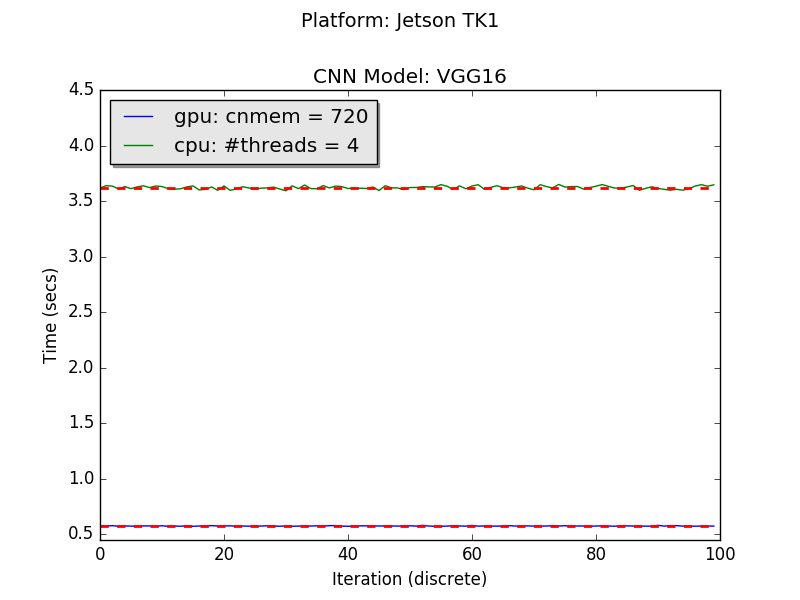
\includegraphics[width=0.8\textwidth]{./images/chapter6/benchmark_vgg16_jetson.png}
  \caption[Χρόνoι εκτέλεσης για το δίκτυο VGG16 στο Jetson TK1]{Χρόνoι εκτέλεσης για το δίκτυο VGG16 στο Jetson TK1}
  \label{fig:vgg16_results_jetson}
\end{figure}


%%----------------------------------------------------------------------------

\subsection{Tiny-YOLO}

Οι παράμετροι των πειραμάτων είναι οι εξής:
\begin{itemize}
  \item{Αριθμός επαναλήψεων: 1000}
  \item{Υπολογιστική μονάδα:}
    \begin{itemize}
      \item{CPU: Αριθμός Νημάτων (1, 2, 4, 8)}
      \item{GPU: Με και χωρίς εκ των προτέρων δέσμευση μνήμης (cnmem)}
    \end{itemize}
\end{itemize}

\begin{table}[!ht]
  \begin{center}
    \caption{Μετρήσεις πειραμάτων για το δίκτυο Tiny-YOLO στο Jetson TK1}
    \label{tab:yolo_jetson}
    \small
    \begin{tabular}[center]{ | c | c | c | c | c | }
      \hline
      \rowcolor{Gray}
      Υπολ. Μονάδα & \# νημάτων & cnmem & Χρόνος εκτέλεσης (sec) & Κατ. Ισχύος (Watts) \\
      \hline
      CPU & 1 & N/A & 1.5902 & 6.318\\
      CPU & 2 & N/A & 1.0276 & 8.504\\
      CPU & 4 & N/A & 0.8137 & 11.9\\
      CPU & 8 & N/A & 0.8126 & 11.9\\
      GPU & N/A & None & 0.5543 & 8\\
      GPU & N/A & 400MB & 0.3872 & 8\\
      \hline
    \end{tabular}
  \end{center}
\end{table}

\begin{figure}[!ht]
  \centering
  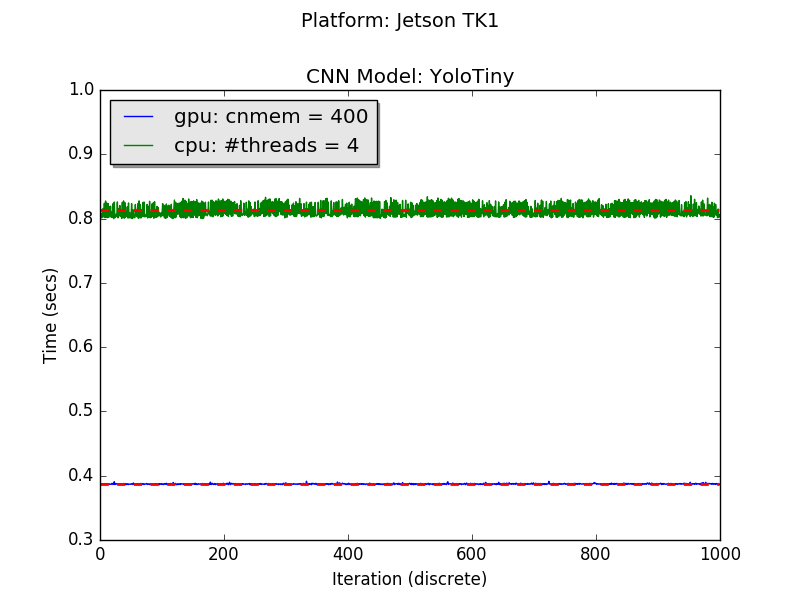
\includegraphics[width=0.8\textwidth]{./images/chapter6/benchmark_yolotiny_jetson.png}
  \caption[Χρόνoι εκτέλεσης για το δίκτυο Tiny-YOLO στο Jetson TK1]{Χρόνοι εκτέλεσης για το δίκτυο Tiny-YOLO στο Jetson TK1}
  \label{fig:yolotiny_results_jetson}
\end{figure}

Ο χρόνος εκτέλεσης της αντίστοιχης υλοποίησης της ερευνητικής ομάδας που
σχεδίασε το δίκτυο Tiny-YOLO μετρήθηκε, για την μονάδα CPU του Tegra K1,
στα 3.475 δευτερόλεπτα (τέσσερις φορές πιο αργό από την υλοποίηση
μας).
Η μέτρηση του χρόνου εκτέλεση της αντίστοιχης
υλοποίησης στην μονάδα GPU ήταν αδύνατη. Η εκτέλεση στην μονάδα GPU
απαιτούσε περισσότερη μνήμη από όση η πλατφόρμα Jetson TK1 διαθέτει και έτσι
το εκτελέσιμο τερματίζει με σφάλμα \emph{CUDA Error: out of memory}.
Ο λόγος που αυτό συμβαίνει μόνο στην περίπτωση εκτέλεσης στην μονάδα GPU
δεν είναι εμφανές. Πιθανόν να σφάλμα τύπου διαρροής μνήμης (memory leak).



\section{Συγκριτικά Αποτελέσματα}
\label{sec:experiments_comparative}

Στον \autoref{tab:results_comparative} συνοψίζονται τα αποτελέσματα που λήφθηκαν στις δύο φάσεις
των πειραμάτων (εκτέλεση σε επεξεργαστή Intel i7-6700 και εκτέλεση στο Jetson TK1).

\begin{table}[H]
  \begin{center}
    \caption{Συγκριτικά αποτελέσματα των πειραμάτων σε επεξεργαστή Intel i7-6700 και το ενσωματωμένο σύστημα Jetson TK1}
    \label{tab:results_comparative}
    \footnotesize
    \begin{tabular}[center]{ | c | c | c | c | c | c | c | }
      \hline
      \rowcolor{Gray}
      CNN & \# Nημάτων & Μονάδα & cnmem & Χρ. Eκτέλεσης & Κατ. Ισχύος & Perf/Watt \\
      \hline
      \multirow{10}{*}{AlexNet}   & \multirow{2}{*}{1}    & i7-6700                     & N/A     & 0.117   & 8.21    & 1.04    \\ \cline{3-7}
                                  &                       & ARM Cortex A15              & N/A     & 0.62    & 6.318   & 0.254   \\ \cline{2-7}
                                  & \multirow{2}{*}{2}    & i7-6700                     & N/A     & 0.095   & 16.43   & 0.64    \\ \cline{3-7}
                                  &                       & ARM Cortex A15              & N/A     & 0.4845  & 8.02    & 0.257   \\ \cline{2-7}
                                  & \multirow{2}{*}{4}    & i7-6700                     & N/A     & 0.095   & 32.62   & 0.32    \\ \cline{3-7}
                                  &                       & ARM Cortex A15              & N/A     & 0.4634  & 10.692  & 0.202   \\ \cline{2-7}
                                  & \multirow{2}{*}{8}    & i7-6700                     & N/A     & 0.127   & 58.84   & 0.13    \\ \cline{3-7}
                                  &                       & ARM Cortex A15              & N/A     & 0.4646  & 10.692  & 0.201   \\ \cline{2-7}
                                  & \multirow{2}{*}{N/A}  & \multirow{2}{*}{GK20a GPU}  & 0       & 0.1049  & 8.5     & 1.121   \\ \cline{4-7}
                                  &                       &                             & 700MB   & 0.1     & 8.5     & 1.176   \\ \hline
      \multirow{10}{*}{VGG16}     & \multirow{2}{*}{1}    & i7-6700                     & N/A     & 0.7709  & 8.26    & 0.157   \\ \cline{3-7}
                                  &                       & ARM Cortex A15              & N/A     & 9.431   & 6.813   & 0.0167  \\ \cline{2-7}
                                  & \multirow{2}{*}{2}    & i7-6700                     & N/A     & 0.5577  & 15.78   & 0.113   \\ \cline{3-7}
                                  &                       & ARM Cortex A15              & N/A     & 5.4476  & 8.748   & 0.021   \\ \cline{2-7}
                                  & \multirow{2}{*}{4}    & i7-6700                     & N/A     & 0.4734  & 29.75   & 0.071   \\ \cline{3-7}
                                  &                       & ARM Cortex A15              & N/A     & 3.6224  & 13.122  & 0.021   \\ \cline{2-7}
                                  & \multirow{2}{*}{8}    & i7-6700                     & N/A     & 0.6555  & 58.97   & 0.025   \\ \cline{3-7}
                                  &                       & ARM Cortex A15              & N/A     & 3.6308  & 13.122  & 0.021   \\ \cline{2-7}
                                  & \multirow{2}{*}{N/A}  & \multirow{2}{*}{GK20a GPU}  & 0       & 0.6983  & 11.907  & 0.1207  \\ \cline{4-7}
                                  &                       &                             & 720MB   & 0.5761  & 11.907  & 0.1457  \\ \hline
      \multirow{10}{*}{TinyYOLO}  & \multirow{2}{*}{1}    & i7-6700                     & N/A     & 0.1871  & 8.23    & 0.65    \\ \cline{3-7}
                                  &                       & ARM Cortex A15              & N/A     & 1.5902  & 6.318   & 0.1     \\ \cline{2-7}
                                  & \multirow{2}{*}{2}    & i7-6700                     & N/A     & 0.1609  & 16.39   & 0.38    \\ \cline{3-7}
                                  &                       & ARM Cortex A15              & N/A     & 1.0276  & 8.5     & 0.1144  \\ \cline{2-7}
                                  & \multirow{2}{*}{4}    & i7-6700                     & N/A     & 0.1516  & 32.7    & 0.2     \\ \cline{3-7}
                                  &                       & ARM Cortex A15              & N/A     & 0.8137  & 11.9    & 0.103   \\ \cline{2-7}
                                  & \multirow{2}{*}{8}    & i7-6700                     & N/A     & 0.2309  & 61.17   & 0.07    \\ \cline{3-7}
                                  &                       & ARM Cortex A15              & N/A     & 0.8126  & 11.9    & 0.1034  \\ \cline{2-7}
                                  & \multirow{2}{*}{N/A}  & \multirow{2}{*}{GK20a GPU}  & 0       & 0.5543  & 8       & 0.2255  \\ \cline{4-7}
                                  &                       &                             & 400MB   & 0.3872  & 8       & 0.323   \\
      \hline
    \end{tabular}
  \end{center}
\end{table}


Οι μετρήσεις κατανάλωσης ισχύος για το ενσωματωμένο σύστημα Jetson TK1 αφορούν την
κατανάλωση σε όλη την πλακέτα, δηλαδή TK1 SoC (CPU + CPU), RAM, ενεργοποιημένες περιφερειακές μονάδες,
απώλειες σε μονάδες μετατροπής τάσης, κα.
Αντιθέτως, οι αντίστοιχες μετρήσεις του παρουσιάζονται για το σύστημα με τον
επεξεργαστή Intel i7-6700, αντιστοιχούν στην κατανάλωση μόνο του επεξεργαστή.

